\documentclass{report}

\input{~/latex/template/preamble.tex}
\input{~/latex/template/macros.tex}

\title{\Huge{Chapter 5 Lecture Notes }}
\author{\huge{Matt Warner}}
\date{\huge{}}
\pagestyle{fancy}
\fancyhf{}
\rhead{Chapter 5 - Random Variables and Discrete Probability Distributions}
\lhead{\leftmark}
\cfoot{\thepage}
% \usepackage[default]{sourcecodepro}
% \usepackage[T1]{fontenc}


\pgfpagesdeclarelayout{boxed}
{
  \edef\pgfpageoptionborder{0pt}
}
{
  \pgfpagesphysicalpageoptions
  {%
    logical pages=1,%
  }
  \pgfpageslogicalpageoptions{1}
  {
    border code=\pgfsetlinewidth{1.5pt}\pgfstroke,%
    border shrink=\pgfpageoptionborder,%
    resized width=.95\pgfphysicalwidth,%
    resized height=.95\pgfphysicalheight,%
    center=\pgfpoint{.5\pgfphysicalwidth}{.5\pgfphysicalheight}%
  }%
}

\pgfpagesuselayout{boxed}

\begin{document}
  \maketitle
  \section*{5.2 - Probability Distributions for Descrete Random Variables}
  \bigbreak \noindent \bigbreak \noindent
  \begin{minipage}{0.5\textwidth}
    \large{\centerline{Chapter 4}}
    \bigbreak \noindent
  \begin{itemize}
    \item Samples space = S = the set of all possible outcomes from an experiment 
    \item Events (Written as A,B,C,etc.) were subsets of outcomes from a sample space
    \item NEw events were formed by using the operations $\cup$ (union), $\cap$ (intersection).  \\ and $^{\complement}$ (complement).  
    \item P(A) = the probabilty that some outcome (or any outcome) in the event would occur
  \end{itemize}	
  \end{minipage}
  \begin{minipage}{0.5\textwidth}
    \large{\centerline{Now}}
    \bigbreak \noindent
    \begin{itemize}
      \item We will express our work using random variables 
      \item \textbf{Random variable} (written as X) is a variable whose possible values are determined by random chance. (The possible values of X are numerical outcomes of a random phenomenon)
      \item 2 types of random variables
    \end{itemize}
        \begin{itemize}[label=$\circ$]
          \item \textbf{Discrete} - values of X are typically whole numbers such as 0,1,2,3,etc. \\ (usually associated with counting, e.g., ``the number of'')
          \item \textbf{Continuous} - values of X are typically every value from an interval on the number line \\ (usually associated with measuring, e.g., heights, weights, times, etc.)
        \end{itemize}
  \end{minipage}
  \bigbreak \bigbreak
\hrule
\bigbreak \noindent
\q
\bigbreak \noindent
   let the discrete random variable X = the roll of an unbalanced or unfair or rigged die, suppose the probability distribution of X is given by the following table.
   \bigbreak \noindent
   \begin{center}
\begin{tabular}{c|cccccc}
$x$ & 1 & 2 & 3 & 4 & 5 & 6 \\
\hline$p(x)$ & 0.40 & 0.20 & 0.12 & 0.10 & 0.14 & $?$
\end{tabular}
\end{center}
   \bigbreak \noindent \bigbreak \noindent
   \nt{
     \begin{itemize}
       \item X would be \textbf{discrete} because its possible values are the whole numbers 1, 2, 3, 4, 5, 6
       \item Events are written as $ X = 2, X < 4, 2 \le X, X < 6, etc.$
     \end{itemize}
     \bigbreak \noindent
     \centerline{\textbf{Notation}}
     \bigbreak \noindent
     \begin{center}
      p(x) is shorthand for P(X = x)
      \bigbreak \noindent
      e.g., p(2) = P(X = 2)
     \end{center}
   }
   \pagebreak
   \noindent
   \bigbreak \noindent
   \textbf{Find p(6)}
   \bigbreak \noindent
   That is,

   $$ P(X = 6)$$
  Sum all the other values in the table
   $$ = .40 + .20 + .12 + .10 + .14 = .96$$
   So,

   $$ p(X = 6) = 1 - 0.96$$
   $$ = .04$$
   \bigbreak \noindent
   \hrule
   \bigbreak \noindent
   \textbf{Find} $\mathbf{P(1 < X \le 4)}$
  \bigbreak \noindent
  That is,

  $$ P(2) + P(3) + P(4)$$
  So, 

  $$ P(1 < X \le 4) = .20 + .12 + .10$$

  $$ = 0.42$$
  \bigbreak \noindent
  \hrule
  \bigbreak \noindent
  \textbf{Find the probability that the roll is at least 4}
  \bigbreak \noindent
  That is,
  $$ P(X \ge 4)$$
  So,

  $$P(X \ge 4) = p(4) + p(5) + p(6)$$

  $$ = .10 + .14 + .04$$ 

  $$ = 0.28$$
\bigbreak \noindent
\hrule
\bigbreak \noindent
\begin{center}
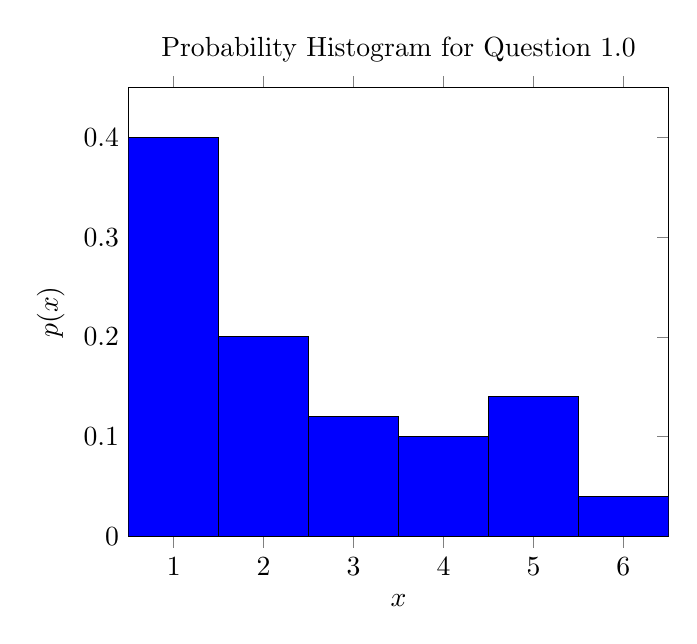
\begin{tikzpicture}
  \begin{axis}[
    ybar,
    ymin=0,
    ymax=0.45,
    xtick=data,
    xticklabels={$1$, $2$, $3$, $4$, $5$, $6$},
    xlabel={$x$},
    ylabel={$p(x)$},
    title={Probability Histogram for Question 1.0},
    bar width=1,
  ]
  \addplot[fill=blue] coordinates {
    (1, 0.40)
    (2, 0.20)
    (3, 0.12)
    (4, 0.10)
    (5, 0.14)
    (6, 0.04) 
  };
  \end{axis}
\end{tikzpicture}
\end{center}
   \pagebreak
   \section*{Section 5.3 - Mean, Variance, and Standard Deviation for a Discrete R.V.} 
   \bigbreak \noindent 
   \subsection*{Important summaries of a \underline{data set} are}
   \bigbreak \noindent
   \begin{itemize}[label=$\circ$]
     \item Sample mean = $\bar{x}$ \hspace{28mm} (This indicates the center of the \textbf{data})
     \item Sample standard deviation = s \hspace{8mm} (This indicates the amount of spread among the \textbf{data})
   \end{itemize}
  \bigbreak \noindent
  Likewise, a random variable or a probability distribution has similar summaries
  \bigbreak \noindent
  \subsection*{Definition}
  Let X be a discrete random variable with probability mass function p(x)
  \bigbreak \noindent
  \begin{itemize}[label=$\circ$]
    \item The \textbf{mean value} ($\mu$) or the \textbf{expected value} (E(X)) of X is
      \bigbreak \noindent
      $$ \text{Symbol}  \hspace{10mm} \text{Calculation}$$
      $$ \hspace{-2mm}\mu \text{ or }E(X) = \sum_{all\ x}\left[x \cdot p(x)\right]$$
  \item The \textbf{variance} of X is
\bigbreak \noindent
    $$ \hspace{-35mm}\text{Symbol}  \hspace{18mm} \text{Calculation}$$
    $$ \sigma^2 \text{ or } Var(X) \ \ =  \ \ \begin{cases}\displaystyle\sum_{all \ x }\left[(x-\mu)^2 \cdot p(x)\right] & \text { (Definition) } \\ E\left(X^2\right)-\mu^2 & \text { (Short Cut) }\end{cases}$$
  \item The \textbf{standard deviation of X is}
  \bigbreak \noindent
    $$ \sigma = \sqrt{\sigma^2}$$
  \end{itemize}
  \bigbreak \noindent
  \nt{
    \begin{itemize}[label=$\circ$]
      \item The mean, $\mu$, gives the value of X that we would expect to see, on average. \\ This indicates the center of a probability histogram
        \bigbreak \noindent
      \item The standard deviation, $\sigma$, measures the amount of spread among the values of X or the amount of spread exhibited by the probability histogram.
        \bigbreak \noindent
      \item If $\sigma$ is
      \begin{itemize}[label=$\bullet$]
        \item Large, then the values of X and/or the probability histogram has more spread
        \item Small, then the values of X and/or the probability histogram has less spread.

        
      \end{itemize}
    \end{itemize}
  }
    \pagebreak
    \q
    \bigbreak \noindent
    Let the discrete random variable X = the roll of an unbalanced or unfair or rigged die. Suppose the probability distribution of X is given by the following table
    \bigbreak \noindent
   \begin{center}
\begin{tabular}{c|cccccc}
$x$ & 1 & 2 & 3 & 4 & 5 & 6 \\
\hline$p(x)$ & 0.40 & 0.20 & 0.12 & 0.10 & 0.14 & 0.04
\end{tabular}
\end{center}
\bigbreak \noindent \bigbreak \noindent
\textbf{Find the mean value of X (also called the expected value of X)}
\bigbreak \noindent
We can use the formula

$$ \displaystyle\sum\left[x \cdot p(x)\right]$$
So,

  $$\mu  = 1(.40) + 2(20)+ 3(.12)+4(.10)+5(.14)+6(.04)$$

  $$= 2.50$$
  \bigbreak \noindent
  \hrule
  \bigbreak \noindent
  \textbf{Find $E(X^2) = \sum\left[x^2 \cdot p(x)\right]$}
    \bigbreak \noindent
    That is,

   $$  1^2(.40) +2^2(.20)+3^2(.12)+ 4^2(.10)+5(.14)+6^2(.04)$$

   $$= 8.82$$
  \bigbreak \noindent
  \hrule
  \bigbreak \noindent
  \textbf{Find the variance of X using the short cut}
  
  $$ Var(X) = E(X^2) - \mu^{2}$$
  So,

  $$ Var(X) = 8.82 - 2.50^{2} = 2.57$$
  \bigbreak \noindent
  \hrule
  \bigbreak \noindent
  \textbf{Find the standard deviation of X}
  \bigbreak \noindent
  Using the formula

  $$ S = \sqrt{S^2}$$
We get

  $$  \sqrt{2.57} = 1.60$$
\bigbreak \noindent \bigbreak \noindent
\pagebreak
\section*{Section 5.4 - The Binomial Distribution}
\bigbreak\noindent
\subsection*{Binomial Experiment} - Any experiment or situation that satisfies the following
\vspace{2mm}

\begin{itemize}
  \item There is a known number of trials (denoted by n) 
  \item Each trial results in a success or a failure
  \item P(success) is the same for every trial (denoted by p)
  \item The trials are independent. That is, the outcome of one trial wil not influence or affect the outcome of another trial
\bigbreak \noindent
\nt{
  The values of $n$ and $p$ are called the \textbf{parameters} of the Binomial experiment
}
\end{itemize}
\bigbreak \noindent
\subsection*{Binomial Random Variable}
\begin{itemize}
  \item X = the total number of success oberserved during a Binomial experiement 
  \item Possible values of X are 0, 1, 2, 3, $\ldots$, n
\end{itemize}
\bigbreak \noindent
\hrule
\bigbreak \noindent
\q
\bigbreak \noindent
\textbf{For each of the following decide whether or not the random variable is a Binomial random variable}
  \bigbreak \noindent
  \begin{enumerate}
    \item A particular variety of seed has an 80\% germination rate. 
      
      \noindent Let X = the number of seeds out of ten that germinate
      \vspace{2mm}

      \subitem  - n = number of seeds (10), 
      \vspace{2mm}

      \subitem - each seeds has either a success or failure (germinating or not)  
      \vspace{2mm}

      \subitem - $p = .80$ (probability of success (germinating). This is also the same $p$ value for every trial ) 
      \vspace{2mm}

      \subitem - seeds are independent
      \vspace{2mm}
      
      \subitem So yes, This is a Binomial random variable

    \item Five cards are drawn without replacement from a deck.

      Let X = the number of red cards drawn
      \vspace{2mm}

      \subitem - n = 5 cards 
      \vspace{2mm}

      \subitem - there does exist either a success or failure 
      \vspace{2mm}

      \subitem - p is not the same everytime since the cards are not replaced.
      \vspace{2mm} 

      \subitem  - this also means that the cards are not independent
      \vspace{3mm}

      \subitem Therefore, this is not a binomial random variable.

    \item  You take a multiple choice quiz with five questions, each containing choices (a) to (d), by guessing

      Let X = the number of correct answers
      \vspace{2mm}

      \subitem - n = 5 
      \vspace{2mm}

      \subitem - each trial does have a success or failure
      \vspace{3mm}
  
      \subitem Therefore, this is not a binomial random variable
  \end{enumerate}
  \bigbreak \noindent
  \hrule
  \bigbreak \noindent
  \subsection*{Binomial Probability Mass Function} 
  \begin{itemize}
  \item $X\sim Bin(n,p)$ means that X is a Binomial random variable with parameters $n$ and $p$
    \item $p(x)$ = the probability of obtaining exactly x successes among the $n$ trials
      $$ = {n \choose x} \cdot p^x \cdot (1-p)^{n-x}$$
      Where

      $$ {n \choose x} = n \text{ choose } x = \dfrac{n!}{x!(n-x)!}$$

      $$ n! = n \cdot (n-1) \cdot (n-2) \ldots 2 \cdot 1$$
  \end{itemize}
  \bigbreak \noindent
  \hrule
  \bigbreak \noindent
  \q
  \bigbreak \noindent
  \textbf{Suppose that you take a multiple choce quiz with $n = 5$ questions, each containing choices (a) to (d), by guessing (so that $p = 0.25$). Let X = the number of correct answers. Here we know that $X \sim Bin(n=5,p=0.25)$}
  \bigbreak \noindent
  \textbf{Find the probability of getting exactly one correct answer. }
  \bigbreak \noindent
That is, 
$$P(X = 1 ) $$
Using the formula

$${n \choose x}\cdot p^x \cdot (1-p)^{n-x}$$
We get

$${5 \choose 1}(.25)(1-.25)^{5-1} = \frac{5!}{1!(5-1)} \cdot 0.25^1 \cdot 0.75^4$$

$$ P(X = 1) = .3955$$ 
\bigbreak \noindent
\hrule
\bigbreak \noindent
\textbf{Find the probability of getting exactly two correct answers}
\bigbreak \noindent
That is
$$P(x = 2)$$
So,

$${5 \choose 2}.25^2(1-.25)^{5-2} = \frac{5!}{2!(5-2)!}  \cdot 0.25^2 \cdot 0.75^3 = 10 \cdot 0.25^2 \cdot 0.75^3 = 0.2637$$

\pagebreak
\noindent
\textbf{Find the probability of getting at most one correct answer}
\bigbreak \noindent
That is

$$ P(X \le 1)$$ 
This equates to

$$ P(x=0) + P(x=1)$$
So,

$${5 \choose 0}0.25^0(1-.25)^{5-0} + {5 \choose 1}(0.25)(0.75)^4 = P(x \le 1)$$

$$ .2373 + .3955 = P(X \le 1)$$

$$ P(X \le 1) = 0.6328$$
\bigbreak \noindent
\hrule
\bigbreak \noindent
\textbf{Find the probability of getting at least four correct answers}
\bigbreak \noindent
That is

$$ P(x\ge 4) $$
$$= P(x=4) + P(x=5)$$
So,

$$ P(x=4) = \frac{5!}{4!1!}0.25^4 \cdot .75^1$$

$$P(x=5) = \frac{5!}{5!0!}0.25^5\cdot0.75^0$$

$$ = .0146 + .0010 = .0156$$
\bigbreak \noindent
\hrule
\bigbreak \noindent
\q
\bigbreak \noindent
\textbf{Suppose that} $\mathbf{X \sim Bin(15,0.40)}$. \textbf{Use the tables of Binomial Distribution Cumulative Probabilities to find each of the following}
  $$ n = 15, \hspace{10mm} p = 0.40$$
  \bigbreak \noindent
a) $P(X \le 7) = 0. 787$
\bigbreak \noindent
b) $P(X >  5) = \text{ using the table, we see that P(X $\le$ 15 ) = 1, and P(X$ < 5$ = .403) so, P( X $>$ 5 = .597)}$
\bigbreak \noindent
c) P( X $ \le $) = .027
\bigbreak \noindent
d) P($2 < x \le 6)$ = P(X $\le$  6) - P($ X \le 2)$ = .610 - .027 = .583
\bigbreak \noindent
e) P($ 5 \le X \le 9)$ = .966 - .217 = .749
\bigbreak \noindent
f) P($ 3 < X < 7)$ = P(X $< $7) - P($ X < 3)$ = .610 - .091 = .519
\bigbreak \noindent
g) P($X = 4)$ .217 - .091 = .126
\bigbreak \noindent
\bigbreak \noindent
\subsection*{Binomial Mean, Variance, \& Standard Deviation} - If X $\sim Bin(n,p)$ then,
\begin{itemize}
  \item Mean: 
    $$ \mu = n\cdot p$$
  \item Variance:
    $$ \sigma^2 = n\cdot p \cdot (1-p)$$
  \item Standard Deviation:
    $$ \sigma = \sqrt{n\cdot p \cdot (1-p)}$$
\end{itemize}
\q
\bigbreak \noindent
\textbf{Suppose that you take a multiple choice quiz with n }
\bigbreak \noindent
A) \textbf{How many questions would you expect to get correct, i.e., what is the mean value of X}
\bigbreak \noindent
Using the formula

$$ \mu = np$$
We get

   $$n \cdot p = 5(.25) $$
   $$= 1.25$$

  \bigbreak \noindent
  \textbf{Find the standard deviation of the number of correct answers}
  \bigbreak \noindent
  First we find the variance

$$  \sigma^2 = np(1-p)$$
$$= 5(.25)(.75)$$
$$ = .9375$$
Now we can find the Standard Deviation
$$ \sigma = \sqrt{.9375}$$
$$ = .9682$$
\pagebreak
\section*{Summary - Using the Binomial Tables}
\bigbreak \noindent
Probability mass function for the Binomial distribution
$$ p(x) = {n \choose x} \cdot p^{x} \cdot (1-p)^{n-x} \hspace{10mm} \text{for x = 0,1,2,\ldots,n}$$
\bigbreak \noindent
The probability mass function is used to calculate the probability of exactly a successes, 
$$ P(X = a)$$
\bigbreak \noindent
However, the Binomial tables are cummulative tables that provide the probability of at most a successes,
$$ P(X \le a)$$
\bigbreak \noindent
Below is a summary of how to use the tables to obtain various probabilities. You should study these until you understand them . They are not on the formula sheet and won't be provided at the exams.
\bigbreak \noindent
\begin{mdframed}
  
\begin{itemize}[label=$\bullet$]
  \item $P(X \le a)$ = table entry for $a$
  \bigbreak
  \item $P(X < a)$ = $P(X \le a - 1)$ \hspace{39mm} e.g. $P(X < 5) = P(X \le 4)$
  \bigbreak
  \item $P(X \ge a) = 1 - P(X \le a -1)$ \hspace{33.5mm} e.g. $P(X \ge 5) = 1 - P(X \le 4)$
  \bigbreak
  \item $P(x > a) = 1 - P(X \le a)$ \hspace{41mm} e.g. $P(X > 5) = 1 - P(X \le 5)$
  \bigbreak
  \item $P(X = a) = P(X \le a) - P(X \le a - 1)$ \hspace{20mm} e.g. $P(X = 5) = P(X \le 5) - P(X \le 4)$
  \bigbreak
  \item $P(X \neq a) = 1-P(X = a)$ 
  \bigbreak
  \item $P(a < X \le b) = P(X \le b) - P(X \le a)$ \hspace{21mm} e.g. $ P(2 < X \le 5) = P(x \le 5) - P(X \le 2)$
  \bigbreak
  \item $P(a \le X \le b) = P(X \le b) - P(X \le a - 1)$ \hspace{15.5mm} e.g. $P(2 \le X \le 5) = P(X \le 5) - P(X \le 1)$
  \bigbreak
  \item $P(a \le X < b) = P(X \le b- 1) - P(X \le a -1)$ \hspace{10mm} e.g. $P(2 \le X < 5) = P(X \le 4) - P(X \le 1)$
  \bigbreak
  \item $P(a < X < b) = P(X \le b - 1) - P(X \le a)$ \hspace{16mm} e.g. $P(2 < X < 5 ) = P(X \le 4) - P(X \le 2)$
\end{itemize}
\end{mdframed}
\end{document}
